\chapter{Performance Results of Catastrophic Forgetting Mitigation Techniques}\label{ch:results}

\par In the following chapter, the results of the implemented Catastrophic Forgetting mitigation techniques will be explored. There are three main categories of results collected: MATLAB simulation results, C++ simulation results, and C++ flight test results. %\textbf{\textit{[ a little bit more here]}}
\section{MATLAB Simulation Results}
\par MATLAB was initially used in developing the modified CEs, both with the RLM training method (CE-RLM) and the Learn++.NSE training method (CE-NSE). The intent of the MATLAB simulation was to verify the potential benefit of both changes to the CE, in an environment where implementing iterational modifications is as frictionless as possible. More realistic analysis, including timing analysis, was conducted in the C++ CE implementation. As such, the SNR profile used in MATLAB-based testing was a simple slow-fading channel, so that degenerate behavior would be definitively a result of poorly implemented code. A plot of the SNR profile is shown in Figure \ref{fig:matlabSNRProf}. 
\begin{figure}[ht]
\centering
\includegraphics[width=\linewidth]{figures/matlab_sim_results/snrPRofile_matlabsim.eps}
\caption{SNR profile used in MATLAB simulation.}
\label{fig:matlabSNRProf}
\end{figure}
\par While there are six different fitness score weightings (as shown in Table \ref{table:fitMissions}), the flight tests conducted in \cite{tim_implementation_paper} focused on Emergency, Cooperation and Power Saving. Because of this, these were the missions that the MATLAB simulation focused on as well. Figure \ref{res:matSimFitscore} shows how the fitness score evolved over time during the simulation.

%\begin{minipage}{0.5\textwidth}
\begin{figure}[ht]
\begin{center}
\begin{subfigure}{\linewidth}
\centering
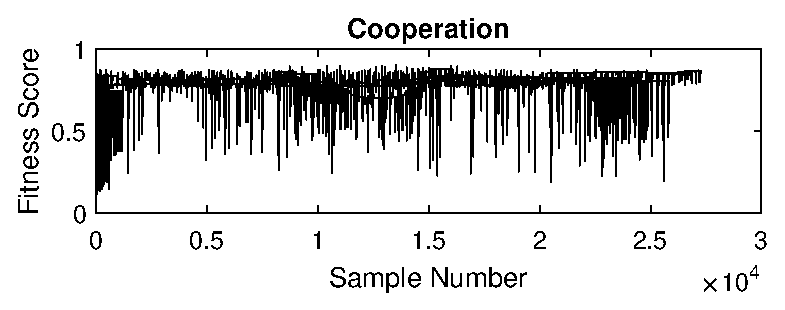
\includegraphics[width=\linewidth]{figures/matlab_sim_results/fitObserved_coop.eps}
\caption{Fitness score plotted over length of simulation, Cooperation mission.}\label{res:matSimFitscore_coop}
\end{subfigure}
\end{center}

\begin{center}
\begin{subfigure}{\linewidth}		
\centering
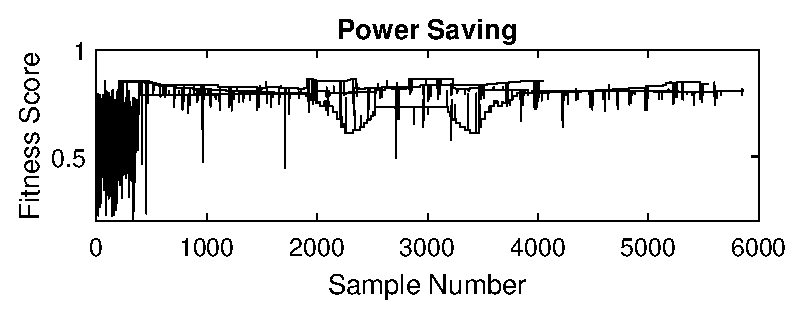
\includegraphics[width=\linewidth]{figures/matlab_sim_results/fitObserved_powerSave.eps}
\caption{Fitness score plotted over length of simulation, Power Saving mission.}\label{res:matSimFitscore_power}
\end{subfigure}
\end{center}

\begin{center}
\begin{subfigure}{\linewidth}
	\centering
	\includegraphics[width=\linewidth]{figures/matlab_sim_results/fitObserved_emer.eps}
\caption{Fitness score plotted over length of simulation, Emergency mission.}\label{res:matSimFitscore_emer}
\end{subfigure}
\end{center}
\caption{Fitness score plotted over length of simulation.}\label{res:matSimFitscore}
\end{figure}
%\end{minipage}

%\begin{minipage}{0.5\textwidth}

%\end{minipage}
\par A few things are worth bringing up with the time series plots shown in Figure\ref{res:matSimFitscore}. The first is that the spurs that are periodically showing up are the CE exploring random actions, and are spaced in a manner independent of training type. Instead, the spacing is solely dependent on the value of the exploration parameter $\epsilon$. In addition, it is apparent that some mission types have different ranges of fitness scores that are possible within the action space, as the Cooperation mission simulation encounters a wider range of values during exploration than either the Emergency mission simulation or the Power Saving mission simulation. Beyond this, it is evident that LM has a more difficult time than the other two training algorithms in adapting to the higher SNR portions of the simulated pass in both the Cooperation and Power Saving mission cases. Other than this, it's fairly difficult to draw conclusions from these time series plots.
\FloatBarrier
\begin{figure}[!ht]
\centering
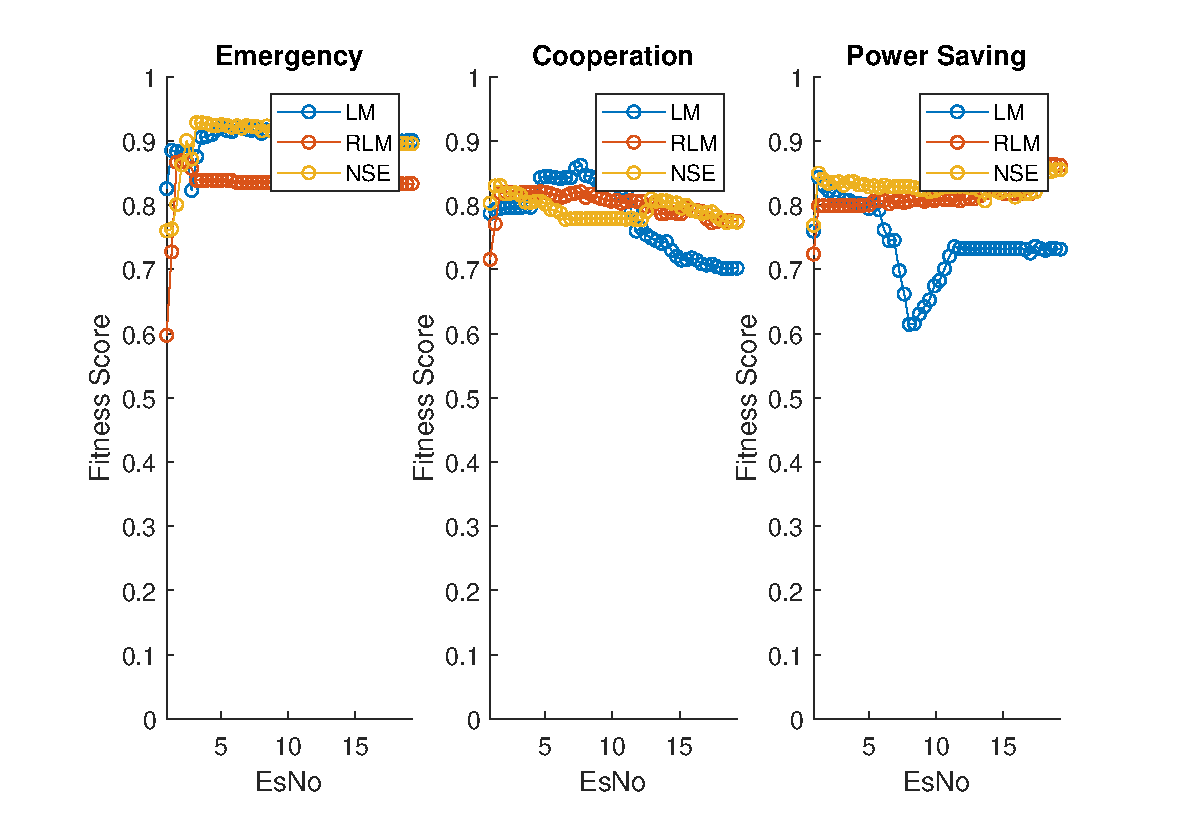
\includegraphics[width=\linewidth]{figures/matlab_sim_results/binnedMeans_sim.eps}
\caption{Binned means, MATLAB simulation}
\label{res:matSimBinMean}
\end{figure}
\par In order to get a better understanding of the behavior of the different modifications of the CE, fitness scores were split into bins based on the $E_s/N_0$ at the moment that the fitness score was observed. Once this was done, the mean was taken within each bin. This plot is shown in Figure \ref{res:matSimBinMean}. For the Emergency mission, CE-LM and CE-NSE proved to have similar mean fitness scores, with CE-RLM having lower mean fitness scores. The Cooperation mission was more ambiguous, with CE-RLM and CE-NSE performing better than CE-LM in the higher $E_s/N_0$ regime, and performing worse than LM in the middle $E_s/N_0$ regime. Finally, the Power Saving mission shows both CE-LM and CE-RLM working markedly better than CE-LM in the entire regime.

\par With the results shown in this section, there was enough motivation to progress from the MATLAB simulation to simulation, ground testing, and flight testing in C++.
\FloatBarrier 
\section{C++ Simulation Results}
\par Simulations using the C++ implementation of the CE served two main purposes. The first purpose of C++ simulations was to verify the correct operation of the code prior to connecting the CE to any hardware. The second purpose is to provide a completely identical $E_s/N_0$ profile with which to compare the different training methods. As much as the NASA flight staff intends to be consistent when evaluating the quality of the communications channel during windows when the ISS is in line of sight, the variation of conditions within each quality category resulted in the different tests conducted between 2017 and 2018 having pass qualities that were hard to directly compare. Running a simulation allows for more direct comparison, albeit without the possibility of shifting the action space in a way that breaks the communication link, preventing an important failure case.
\par The SNR profiles used in the C++ simulation come from attenuation profiles that were measured by NASA employees at GRC. These profiles are used with variable attenuators to simulate channel conditions. By subtracting values in these profiles from the maximum $E_s/N_0$ that the CE is expected to see, the attenuation is transformed into suitable $E_s/N_0$ values. These values were fed to the CE. One example snrProfile is shown in Figure \ref{fig:cSimSNRProfile}, while the rest can be found in Appendix \ref{app:cTimeSeries}. 

\begin{figure}[ht]
\centering
\includegraphics[width=\textwidth]{figures/c_sim_timeSeries/EsNo_profile_LM_coop_24.eps}
\caption{One of the SNR profiles used in C++ simulation.}
\label{fig:cSimSNRProfile}
\end{figure}
\FloatBarrier
\par The $E_s/N_0$ profiles for the C++ simulation are significantly more complex than the $E_s/N_0$ profile used in the MATLAB simulation. This is because the slow fading channel simulated in MATLAB is oversimplified for the case of satellite communications. One of the key differences between CE-LM and the new methods being studied is that both CE-RLM and CE-NSE can get added value from pretraining. RLM can explicitly learn a better representation of the environment, while Learn++.NSE can build up a cache of pretrained networks. LM, on the other hand, will replace the information learned in pretraining upon the first retraining period, and so CE-LM did not utilize pretraining. 
\par Running the C++ CE implementation generates a logging file, containing the salient information from each iteration of the algorithm, including the time it takes to choose an action, the fitness score observed, and the other evaluation metrics that combine to become the fitness score. Figure \ref{fig:c22LMCoop} is a summary plot of CE-LM running LM operating the Cooperation mission on the SNR profile shown in Figure \ref{fig:cSimSNRProfile}. The same plots for CE-RLM and CE-NSE are shown in Figures \ref{fig:c22RLMCoop} and \ref{fig:c22NSECoop} respectively. The key difference that's noticable from this series of plots is that RLM takes a significantly longer amount of time to train, as expected. The plots also provide some intuition about what the action space is actually representing. Even with this, this set of visualizations is hard to utilize for comparing training methods.
\begin{figure}[ht!]
\centering
\begin{subfigure}{\linewidth}
	\centering
	\includegraphics[width=\textwidth]{figures/c_sim_timeSeries/EsNo_profile_LM_coop_22.eps}
	% \caption{SNR Profile}
\end{subfigure}\\
\begin{subfigure}{\linewidth}
	\centering
	\includegraphics[width=\textwidth]{figures/c_sim_timeSeries/Fitness_timeSeries_LM_coop_22.eps}
	% \caption{Fitness Observed}
\end{subfigure}\\
\begin{subfigure}{\linewidth}
	\centering
	\includegraphics[width=\textwidth]{figures/c_sim_timeSeries/subfit_emerPriority_LM_coop_22.eps}
	% \caption{Subfitness observed, Throughput and FER}
\end{subfigure}\\
\begin{subfigure}{\linewidth}
	\centering
	\includegraphics[width=\textwidth]{figures/c_sim_timeSeries/subfit_coopPriority_LM_coop_22.eps}
	% \caption{Subfitness observed, Bandwidth and Spectral Efficiency}
\end{subfigure}\\
\begin{subfigure}{\linewidth}
	\centering
	\includegraphics[width=\textwidth]{figures/c_sim_timeSeries/subfit_pwrPriority_LM_coop_22.eps}
	% \caption{Subfitness observed, TX Power Efficiency and Power Consumption}
\end{subfigure}\\
\caption{Operation of CE-LM on SNR profile 22, using the Cooperation mission. Includes SNR profile, fitness observed, and subfitness values observed.} \label{fig:c22LMCoop}
\end{figure}

\begin{figure}[ht!]
\centering
\begin{subfigure}{\linewidth}
	\centering
	\includegraphics[width=\textwidth]{figures/c_sim_timeSeries/EsNo_profile_RLM_coop_22.eps}
\end{subfigure}\\
\begin{subfigure}{\linewidth}
	\centering
	\includegraphics[width=\textwidth]{figures/c_sim_timeSeries/Fitness_timeSeries_RLM_coop_22.eps}
\end{subfigure}\\
\begin{subfigure}{\linewidth}
	\centering
	\includegraphics[width=\textwidth]{figures/c_sim_timeSeries/subfit_emerPriority_RLM_coop_22.eps}
\end{subfigure}\\
\begin{subfigure}{\linewidth}
	\centering
	\includegraphics[width=\textwidth]{figures/c_sim_timeSeries/subfit_coopPriority_RLM_coop_22.eps}
	
\end{subfigure}\\
\begin{subfigure}{\linewidth}
	\centering
	\includegraphics[width=\textwidth]{figures/c_sim_timeSeries/subfit_pwrPriority_RLM_coop_22.eps}
\end{subfigure}\\
\caption{Operation of CE-RLM on SNR profile 22, using the Cooperation mission. Includes SNR profile, fitness observed, and subfitness values observed.}\label{fig:c22RLMCoop}
\end{figure}

\begin{figure}[ht!]
\centering
\begin{subfigure}{\linewidth}
	\centering
	\includegraphics[width=\textwidth]{figures/c_sim_timeSeries/EsNo_profile_NSE_coop_22.eps}
\end{subfigure}\\
\begin{subfigure}{\linewidth}
	\centering
	\includegraphics[width=\textwidth]{figures/c_sim_timeSeries/Fitness_timeSeries_NSE_coop_22.eps}
\end{subfigure}\\
\begin{subfigure}{\linewidth}
	\centering
	\includegraphics[width=\textwidth]{figures/c_sim_timeSeries/subfit_emerPriority_NSE_coop_22.eps}
\end{subfigure}\\
\begin{subfigure}{\linewidth}
	\centering
	\includegraphics[width=\textwidth]{figures/c_sim_timeSeries/subfit_coopPriority_NSE_coop_22.eps}
	
\end{subfigure}\\
\begin{subfigure}{\linewidth}
	\centering
	\includegraphics[width=\textwidth]{figures/c_sim_timeSeries/subfit_pwrPriority_NSE_coop_22.eps}
\end{subfigure}\\
\caption{Operation of CE-NSE on SNR profile 22, using the Cooperation mission. Includes SNR profile, fitness observed, and subfitness values observed.}\label{fig:c22NSECoop}
\end{figure}
%\clearpage
\clearpage

\par Like the MATLAB simulation, the fitness scores were binned by $E_s/N_0$, and the mean and median were taken within each bin. Unlike the MATLAB simulation, however, the postprocessing of the CE log files includes the calculation of the ideal action to be taken during each iteration, given the last observed state. This was left out of the MATLAB simulation because the training methods use the same SNR profile, and could be compared more directly to each other than results from the flight test. Because the calculation of the ideal action was already built into the postprocessing script, the C++ simulations utilize this ideal action and fitness score in evaluation. Using the ideal fitness score acheivable, the fitness values observed are normalized by subtracting them from the ideal fitness value. This will be referred to as the fitness distance and will replace the raw fitness scores for the majority of the following plots.
\begin{figure}[ht]
\centering
\begin{subfigure}{0.48\linewidth}
\centering
\includegraphics{figures/c_sim_results/Mean_Cooperation_22_trunc.eps}
\caption{Binned mean of fitness distance between ideal fitness and observed fitness.}
\end{subfigure}\hfill%
\begin{subfigure}{0.48\linewidth}
\centering
\includegraphics{figures/c_sim_results/Median_Cooperation_22_trunc.eps}
\caption{Binned median of fitness distance between ideal fitness and observed fitness.}
\end{subfigure}
\caption{Binned mean and binned median plots for the different CE training methods running the Cooperation mission. Both the mean and median are derived by binning the fitness scores by the $E_s/N_0$ values observed at the same time as the scores, then getting the mean or median within each bin.} \label{fig:cSimBinMeanMedCoop}
\end{figure}


\par The binned mean and median plots are shown in Figure \ref{fig:cSimBinMeanMedCoop}. The first notable observation is that CE-RLM performed significantly worse than either CE-LM or CE-NSE. This behavior may be attributed to the RLM algorithm requiring more training iterations to properly converge vs the other algorithms, which combined with the extended time it takes to train is resulting in non-convergence. %% TODO: check this 
This non-convergence seems to be situational to individual pass/performance combinations. For instance, running the Power Saving mission on the same $E_s/N_0$ profile results in CE-RLM outperforming CE-NSE and CE-LM. This is shown in Figure \ref{fig:cSimBinMeanMedPwr}. In this case, CE-RLM likely converged.   

\begin{figure}[ht]
\centering
\begin{subfigure}{0.48\linewidth}
\centering
\includegraphics{figures/c_sim_results/Mean_Powersaving_22_trunc.eps}
\caption{Binned mean of fitness distance between ideal fitness and observed fitness.}
\end{subfigure}\hfill%
\begin{subfigure}{0.48\linewidth}
\centering
\includegraphics{figures/c_sim_results/Median_Powersaving_22_trunc.eps}
\caption{Binned median of fitness distance between ideal fitness and observed fitness.}
\end{subfigure}
\caption{Binned mean and binned median plots for the different CE training methods running the Power Saving mission. Both the mean and median are derived by binning the fitness scores by the $E_s/N_0$ values observed at the same time as the scores, then getting the mean or median within each bin.} \label{fig:cSimBinMeanMedPwr}
\end{figure}

\par The binned mean and median representations allow for a simple evaluation of performance between the training methods, but is potentially an oversimplification, collapsing multiple CE behaviors into one number. A different representation of the data is shown in Figure \ref{fig:cSimBin2dHist}. In this figure, a 2-dimensional histogram is taken. One dimension is the $E_s/N_0$ bins, in the same way as the binned means plot previously. The other dimension is the fitness distance observed. The counts are then put on a log scale. This style of plot makes it easier to understand what the CE is actually doing. Each visible line represents an action or cluster of actions selected by the CE. At lower $E_s/N_0$ values, these actions often approach the best action that can be taken. When the CE has identified an action that functions well, it tends to not explore far enough to locate one that may work better. This results in the same action continuing to be chosen for higher $E_s/N_0$ values, where it's performance may not be as close to the ideal one, despite being close to ideal at lower $E_s/N_0$ values. The consistent bar of high fitness distance actions in the plots represent the failure case of the CE, when the action chosen reports zero fitness. The repeated zero fitness score iterations potentially skew the mean of any binned mean values. Binned Medians are also included, in order to reduce the impact of the zero-based skew. More of these plots are shown in Appendix \ref{app:2dHistSim}.

\begin{figure}[ht]
\begin{subfigure}{0.30\linewidth}
	\centering
	\includegraphics[scale=0.9]{figures/c_sim_results/LM_22_Cooperation_2dHist_trunc.eps}
	\caption{CE-LM}
	\label{fig:cSim2dHist_LM}
\end{subfigure}\hfill%
\begin{subfigure}{0.30\linewidth}
	\centering
	\includegraphics[scale=0.9]{figures/c_sim_results/RLM_22_Cooperation_2dHist_trunc.eps}
	\caption{CE-RLM}
	\label{fig:cSim2dHist_RLM}
\end{subfigure}\hfill%
\begin{subfigure}{0.30\linewidth}
	\centering
	\includegraphics[scale=0.9]{figures/c_sim_results/NSE_22_Cooperation_2dHist_trunc.eps}
	\caption{CE-NSE}
	\label{fig:cSim2dHist_NSE}
\end{subfigure}
\caption{Two-dimensional histograms of each training method operating the Cooperation mission. The dimensions are ($E_s/N_0$, fitness score, $log_10($number of frames observed$)$} \label{fig:cSimBin2dHist}
\end{figure}

\par In order to approach a single-number evaluation of the performance of the different training methods, the binned mean fitness distances for each method is compared. For each SNR profile used, the difference is taken between the fitness distances of CE-LM and CE-NSE, and CE-LM and CE-RLM. This difference turns out positive if the first method in the difference has a higher fitness distance than the second method, implying the second method performed better. Likewise, this number is negative if the second method has a higher fitness distance than the first method. The difference in means is then summed up. This is done for each of the simulations, and is shown in Figure \ref{fig:unweight_sumFit}.

\begin{figure}[ht]
\begin{subfigure}{0.30\linewidth}
	\centering
	\includegraphics[scale=0.9]{figures/c_sim_results/sumMeanLM-RLM_Emergency_binnedMean_trunc.eps}
	\caption{CE-LM - CE-RLM, Emergency mission}
	\label{fig:cSimUnweightEmer_RLM}
\end{subfigure}\hfill%
\begin{subfigure}{0.30\linewidth}
	\centering
	\includegraphics[scale=0.9]{figures/c_sim_results/sumMeanLM-RLM_Cooperation_binnedMean_trunc.eps}
	\caption{CE-LM - CE-RLM, Cooperation mission}
	\label{fig:cSimUnweightCoop_RLM}
\end{subfigure}\hfill%
\begin{subfigure}{0.30\linewidth}
	\centering
	\includegraphics[scale=0.9]{figures/c_sim_results/sumMeanLM-RLM_Powersaving_binnedMean_trunc.eps}
	\caption{CE-LM - CE-RLM, Power Saving mission}
	\label{fig:cSimUnweightPower_RLM}
\end{subfigure}
%%%
\begin{subfigure}{0.30\linewidth}
	\centering
	\includegraphics[scale=0.9]{figures/c_sim_results/sumMeanLM-NSE_Emergency_binnedMean_trunc.eps}
	\caption{CE-LM - CE-NSE, Emergency mission}
	\label{fig:cSimUnweightEmer_NSE}
\end{subfigure}\hfill%
\begin{subfigure}{0.30\linewidth}
	\centering
	\includegraphics[scale=0.9]{figures/c_sim_results/sumMeanLM-NSE_Cooperation_binnedMean_trunc.eps}
	\caption{CE-LM - CE-NSE, Cooperation mission}
	\label{fig:cSimUnweightCoop_NSE}
\end{subfigure}\hfill%
\begin{subfigure}{0.30\linewidth}
	\centering
	\includegraphics[scale=0.9]{figures/c_sim_results/sumMeanLM-NSE_Powersaving_binnedMean_trunc.eps}
	\caption{CE-LM - CE-NSE, Power Saving mission}
	\label{fig:cSimUnweightPower_NSE}
\end{subfigure}%
\caption {A series of bar plots taking unweighted sum of the difference between binned means from CE-LM and either CE-RLM or CE-NSE. (\protect\subref{fig:cSimUnweightEmer_RLM}),(\protect\subref{fig:cSimUnweightCoop_RLM}), and (\protect\subref{fig:cSimUnweightPower_RLM}) are between CE-LM and CE-RLM, while (\protect\subref{fig:cSimUnweightEmer_NSE}),(\protect\subref{fig:cSimUnweightCoop_NSE}), and (\protect\subref{fig:cSimUnweightPower_NSE}) are between CE-LM and CE-NSE.} \label{fig:unweight_sumFit} 
\end{figure}
\clearpage

\par For the Emergency and Cooperation missions, It is fairly clear that CE-NSE outperforms CE-RLM, with the majority of the fitness distance sums being positive. Looking at Figures \ref{fig:c22RLMCoop} and \ref{fig:c22NSECoop}, this appears likely due to the fact that the exploit networks having not properly converged to an action given the $E_s/N_0$ behavior. However, as mentioned before this isn't always the case, as CE-RLM outperforms both CE-LM and CE-NSE for most SNR profiles during the Power Saving mission. For all missions, CE-NSE appears to have modest improvements on the performance of CE-LM overall. The moderate but not overwhelming improvements can be attributed to the fact that the base learning algorithm is the same, and all the improvements come from clever usage of ensembles.


\par One potential flaw of the plots in Figure \ref{fig:unweight_sumFit} is that a bin that has a small number samples in it would have the same impact on the plot as a bin that has a large samples in it. In order to mitigate this, the same plots were recalculated, except the mean and median values of the bins were multiplied by the number of samples in the bin divided by the total number of samples. This way, a good performance in a common $E_s/N_0$ regime won't be overshadowed by a poor performance in an uncommon $E_s/N_0$ regime. These modified plots are shown in Figure \ref{fig:weight_sumFit}. This normalization changed some of the results for individual SNR profiles, but the general patterns observed remain the same.


\begin{figure}[ht]
\begin{subfigure}{0.30\linewidth}
	\centering
	\includegraphics[scale=0.9]{figures/c_sim_results/weightSumMeanLM-RLM_Emergency_binnedMean_trunc.eps}
	\caption{CE-LM - CE-RLM, Emergency mission}
	\label{fig:cSimWeightEmer_RLM}
\end{subfigure}\hfill%
\begin{subfigure}{0.30\linewidth}
	\centering
	\includegraphics[scale=0.9]{figures/c_sim_results/weightSumMeanLM-RLM_Cooperation_binnedMean_trunc.eps}
	\caption{CE-LM - CE-RLM, Cooperation mission}
	\label{fig:cSimWeightCoop_RLM}
\end{subfigure}\hfill%
\begin{subfigure}{0.30\linewidth}
	\centering
	\includegraphics[scale=0.9]{figures/c_sim_results/weightSumMeanLM-RLM_Powersaving_binnedMean_trunc.eps}
	\caption{CE-LM - CE-RLM, Power Saving mission}
	\label{fig:cSimWeightPower_RLM}
\end{subfigure}
%%%
\begin{subfigure}{0.30\linewidth}
	\centering
	\includegraphics[scale=0.9]{figures/c_sim_results/weightSumMeanLM-NSE_Emergency_binnedMean_trunc.eps}
	\caption{CE-LM - CE-NSE, Emergency mission}
	\label{fig:cSimWeightEmer_NSE}
\end{subfigure}\hfill%
\begin{subfigure}{0.30\linewidth}
	\centering
	\includegraphics[scale=0.9]{figures/c_sim_results/weightSumMeanLM-NSE_Cooperation_binnedMean_trunc.eps}
	\caption{CE-LM - CE-NSE, Cooperation mission}
	\label{fig:cSimWeightCoop_NSE}
\end{subfigure}\hfill%
\begin{subfigure}{0.30\linewidth}
	\centering
	\includegraphics[scale=0.9]{figures/c_sim_results/weightSumMeanLM-NSE_Powersaving_binnedMean_trunc.eps}
	\caption{CE-LM - CE-NSE, Power Saving mission}
	\label{fig:cSimWeightPower_NSE}
\end{subfigure}%
\caption {A series of bar plots taking a weighted sum of the difference between binned means from CE-LM and either CE-RLM or CE-NSE. (\protect\subref{fig:cSimWeightEmer_RLM}),(\protect\subref{fig:cSimWeightCoop_RLM}), and (\protect\subref{fig:cSimWeightPower_RLM}) are between CE-LM and CE-RLM, while (\protect\subref{fig:cSimWeightEmer_NSE})(,\protect\subref{fig:cSimWeightCoop_NSE}), and (\protect\subref{fig:cSimWeightPower_NSE}) are between CE-LM and CE-NSE.} \label{fig:weight_sumFit} 
\end{figure}
\clearpage



\section{Real-World Flight Test Results}
\par Flight tests were conducted in two different time periods: the testing of CE-LM were conducted between May 2, 2017 and May 12, 2017, as described in \cite{tim_implementation_paper}, while the testing of CE-RLM and CE-NSE took place between August 16, 2018 and August 24, 2018. Tables containing more details about the conditions in which the training methods were tested are included in Appendices \ref{app:pass_details_2017} and \ref{app:pass_details_2018}. 
\par The quality of passes were split into qualitative categories: Excellent/Great, Good, and OK/Poor. Excellent and Great (as well as OK and Poor) are separate categories, but have been combined during processing as a result of the limited amount of time for testing. As stated previously, these categories were determined by the NASA flight staff, and were related to the amount of time where the $E_s/N_0$ was above certain thresholds. Observed $E_s/N_0$ profiles representing each category are shown in Figure \ref{fig:snrProfileVarieties_flight}.
\begin{figure}[ht!]
\centering
\begin{subfigure}{\linewidth}
\centering
\includegraphics{figures/flight_results/EsNo_profile_coop_great_NSE.eps}
\caption{$E_s/N_0$ observerd during flight test II-24, classified as Great.}
\end{subfigure}
\begin{subfigure}{\linewidth}
\centering
\includegraphics{figures/flight_results/EsNo_profile_coop_good_NSE.eps}
\caption{$E_s/N_0$ observerd during flight test II-23, classified as Good.}
\end{subfigure}
\begin{subfigure}{\linewidth}
\centering
\includegraphics{figures/flight_results/EsNo_profile_coop_poor_NSE.eps}
\caption{$E_s/N_0$ observerd during flight test II-19, classified as Poor.}
\end{subfigure}

\caption{$E_s/N_0$ profiles observed with each category label.} \label{fig:snrProfileVarieties_flight}
\end{figure} 

\clearpage

\par Overview plots of CE-LM, CE-RLM, and CE-NSE are shown in Figures \ref{fig:flight_lm_coop_great_overview},\ref{fig:flight_rlm_coop_great_overview} and \ref{fig:flight_nse_coop_great_overview}, respectively. Like before, it is a bit challenging to make significant statements based on these plots, made even more difficult by the fact that the passes are no longer directly comparable. Nonetheless, there are still a few things to be observed. First of all, in the first portion of the pass (roughly from 0-150 s), CE-LM and CE-NSE both are stable in the action chosen, which improves in fitness score as the $E_s/N_0$ improves. This is unlike CE-RLM, which appears to periodically get dislodged from an action by a variation in the $E_s/N_0$'s trend upwards. These same patterns do not impact CE-LM or CE-NSE. The next significant portion of the pass (250-500 s) maintains the same behavior from CE-RLM, while CE-LM and CE-NSE no longer have a stable action chosen. 

% Fo

\begin{figure}[ht!]
\centering
\begin{subfigure}{\linewidth}
	\centering
	\includegraphics[width=\textwidth]{figures/flight_results/EsNo_profile_coop_great_LM.eps}
\end{subfigure}\\
\begin{subfigure}{\linewidth}
	\centering
	\includegraphics[width=\textwidth]{figures/flight_results/Fitness_timeSeries_coop_great_LM.eps}
\end{subfigure}\\
\begin{subfigure}{\linewidth}
	\centering
	\includegraphics[width=\textwidth]{figures/flight_results/subfit_emerPriority_coop_great_LM.eps}
\end{subfigure}\\
\begin{subfigure}{\linewidth}
	\centering
	\includegraphics[width=\textwidth]{figures/flight_results/subfit_coopPriority_coop_great_LM.eps}
	
\end{subfigure}\\
\begin{subfigure}{\linewidth}
	\centering
	\includegraphics[width=\textwidth]{figures/flight_results/subfit_pwrPriority_coop_great_LM.eps}
\end{subfigure}\\
\caption{Operation of CE-LM during Great quality pass using the Cooperation mission. Includes SNR profile, fitness observed, and subfitness values observed.}\label{fig:flight_lm_coop_great_overview}
\end{figure}

\begin{figure}[ht!]
\centering
\begin{subfigure}{\linewidth}
	\centering
	\includegraphics[width=\textwidth]{figures/flight_results/EsNo_profile_coop_great_RLM.eps}
\end{subfigure}\\
\begin{subfigure}{\linewidth}
	\centering
	\includegraphics[width=\textwidth]{figures/flight_results/Fitness_timeSeries_coop_great_RLM.eps}
\end{subfigure}\\
\begin{subfigure}{\linewidth}
	\centering
	\includegraphics[width=\textwidth]{figures/flight_results/subfit_emerPriority_coop_great_RLM.eps}
\end{subfigure}\\
\begin{subfigure}{\linewidth}
	\centering
	\includegraphics[width=\textwidth]{figures/flight_results/subfit_coopPriority_coop_great_RLM.eps}
	
\end{subfigure}\\
\begin{subfigure}{\linewidth}
	\centering
	\includegraphics[width=\textwidth]{figures/flight_results/subfit_pwrPriority_coop_great_RLM.eps}
\end{subfigure}\\
\caption{Operation of CE-RLM during Great quality pass using the Cooperation mission. Includes SNR profile, fitness observed, and subfitness values observed.}\label{fig:flight_rlm_coop_great_overview}
\end{figure}
\begin{figure}[ht!]
\centering
\begin{subfigure}{\linewidth}
	\centering
	\includegraphics[width=\textwidth]{figures/flight_results/EsNo_profile_coop_great_NSE.eps}
\end{subfigure}\\
\begin{subfigure}{\linewidth}
	\centering
	\includegraphics[width=\textwidth]{figures/flight_results/Fitness_timeSeries_coop_great_NSE.eps}
\end{subfigure}\\
\begin{subfigure}{\linewidth}
	\centering
	\includegraphics[width=\textwidth]{figures/flight_results/subfit_emerPriority_coop_great_NSE.eps}
\end{subfigure}\\
\begin{subfigure}{\linewidth}
	\centering
	\includegraphics[width=\textwidth]{figures/flight_results/subfit_coopPriority_coop_great_NSE.eps}
	
\end{subfigure}\\
\begin{subfigure}{\linewidth}
	\centering
	\includegraphics[width=\textwidth]{figures/flight_results/subfit_pwrPriority_coop_great_NSE.eps}
\end{subfigure}\\
\caption{Operation of CE-NSE during Great quality pass using the Cooperation mission. Includes SNR profile, fitness observed, and subfitness values observed.}\label{fig:flight_nse_coop_great_overview}
\end{figure}
\clearpage
% \begin{figure}[ht]
% \centering
% \includegraphics[width=\textwidth]{figures/flight_results/coop_great_rlm_overview.eps}
% \caption{Overview of CE-RLM operating Cooperation mission on Great quality pass.}
% \label{fig:flight_rlm_coop_great_overview}
% \end{figure}
% \begin{figure}[ht]
% \centering
% \includegraphics[width=\textwidth]{figures/flight_results/coop_great_nse_overview.eps}
% \caption{Overview of CE-NSE operating Cooperation mission on Great quality pass.}
% \label{fig:flight_nse_coop_great_overview}
% \end{figure}


\par Figure \ref{fig:coop_great_2dhist} shows the 2D histograms generated for each training method. Like the C++ simulation, the X dimension of the histogram is the $E_s/N_0$ observed, and the Y dimension is the fitness distance observed. However, unlike the C++ simulation, the colored dimension is the count of samples that fall in that bin normalized by the total count of samples. This is done to mitigate the fact that different passes are likely to have different numbers of frames observed before finishing. In the C++ simulation this normalization was less important because the different training methods all used the same $E_s/N_0$ profile. However, with the flight test results the counts likely to vary by a significant margin

\begin{figure}[ht]
\begin{subfigure}{0.30\linewidth}
	\centering
	\includegraphics[scale=0.9]{figures/flight_results/optFitObs_2dHist_Great_coop_LM.eps}
	\caption{CE-LM}
	\label{fig:coopGreat2dHist_LM}
\end{subfigure}\hfill%
\begin{subfigure}{0.30\linewidth}
	\centering
	\includegraphics[scale=0.9]{figures/flight_results/optFitObs_2dHist_Great_coop_RLM.eps}
	\caption{CE-RLM}
	\label{fig:coopGreat2dHist_RLM}
\end{subfigure}\hfill%
\begin{subfigure}{0.30\linewidth}
	\centering
	\includegraphics[scale=0.9]{figures/flight_results/optFitObs_2dHist_Great_coop_NSE.eps}
	\caption{CE-NSE}
	\label{fig:coopGreat2dHist_NSE}
\end{subfigure}
\caption{Two-dimensional histograms of each training method operating the Cooperation mission on a Great quality pass. The dimensions are ($E_s/N_0$, fitness score, $log_10($number of frames observed/total number of frames$)$} \label{fig:coop_great_2dhist}
\end{figure}

\par Looking at Figure \ref{fig:coop_great_2dhist}, the behavior of each training method becomes clear. CE-RLM performs the worst. It appears to have converged fairly well to an action in the high $E_s/N_0$ regime. It appears to be locked on to this action more so than CE-LM or CE-NSE, which have a wider range of fitness distances observed in the same regime, all with lower fitness distances. Beyond the middle $E_s/N_0$ regime though, it loses any action to be taken, and keeps exploring. CE-NSE performs similarly to CE-LM in the higher $E_s/N_0$ regime and the lower $E_s/N_0$ regime, but has trouble in the middle regime. Comparing Figures \ref{fig:flight_lm_coop_great_overview} and \ref{fig:flight_nse_coop_great_overview}, it's likely that this is because the $E_s/N_0$ changes more rapidly during between 250 and 350 seconds. CE-LM appears to lock on to an action during this time, while CE-NSE does not. 


% \par Figures \ref{fig:flight_lm_coop_good_overview}, \ref{fig:flight_rlm_coop_good_overview}, and \ref{fig:flight_nse_coop_good_overview} are overview plots of CE-LM, CE-RLM, and CE-NSE during "Good" passes. Once again CE-RLM appears to perform worse than CE-LM and CE-NSE. Because of the low quality of the pass between 100 and 150 seconds, CE-RLM forces a retraining. Since the RLM algorithm is implemented sample-by-sample, this retraining is most of the pass. CE-NSE encounters a similar patch, but recovers. 

% \begin{figure}[ht!]
% \centering
% \begin{subfigure}{\linewidth}
% 	\centering
% 	\includegraphics[width=\textwidth]{figures/flight_results/EsNo_profile_coop_good_LM.eps}
% \end{subfigure}\\
% \begin{subfigure}{\linewidth}
% 	\centering
% 	\includegraphics[width=\textwidth]{figures/flight_results/Fitness_timeSeries_coop_good_LM.eps}
% \end{subfigure}\\
% \begin{subfigure}{\linewidth}
% 	\centering
% 	\includegraphics[width=\textwidth]{figures/flight_results/subfit_emerPriority_coop_good_LM.eps}
% \end{subfigure}\\
% \begin{subfigure}{\linewidth}
% 	\centering
% 	\includegraphics[width=\textwidth]{figures/flight_results/subfit_coopPriority_coop_good_LM.eps}
	
% \end{subfigure}\\
% \begin{subfigure}{\linewidth}
% 	\centering
% 	\includegraphics[width=\textwidth]{figures/flight_results/subfit_pwrPriority_coop_good_LM.eps}
% \end{subfigure}\\
% \caption{Operation of CE-LM during Good quality pass using the Cooperation mission. Includes SNR profile, fitness observed, and subfitness values observed.}\label{fig:flight_lm_coop_good_overview}
% \end{figure}


% \begin{figure}[ht!]
% \centering
% \begin{subfigure}{\linewidth}
% 	\centering
% 	\includegraphics[width=\textwidth]{figures/flight_results/EsNo_profile_coop_good_RLM.eps}
% \end{subfigure}\\
% \begin{subfigure}{\linewidth}
% 	\centering
% 	\includegraphics[width=\textwidth]{figures/flight_results/Fitness_timeSeries_coop_good_RLM.eps}
% \end{subfigure}\\
% \begin{subfigure}{\linewidth}
% 	\centering
% 	\includegraphics[width=\textwidth]{figures/flight_results/subfit_emerPriority_coop_good_RLM.eps}
% \end{subfigure}\\
% \begin{subfigure}{\linewidth}
% 	\centering
% 	\includegraphics[width=\textwidth]{figures/flight_results/subfit_coopPriority_coop_good_RLM.eps}
	
% \end{subfigure}\\
% \begin{subfigure}{\linewidth}
% 	\centering
% 	\includegraphics[width=\textwidth]{figures/flight_results/subfit_pwrPriority_coop_good_RLM.eps}
% \end{subfigure}\\
% \caption{Operation of CE-RLM during Good quality pass using the Cooperation mission. Includes SNR profile, fitness observed, and subfitness values observed.}\label{fig:flight_rlm_coop_good_overview}
% \end{figure}

% \begin{figure}[ht!]
% \centering
% \begin{subfigure}{\linewidth}
% 	\centering
% 	\includegraphics[width=\textwidth]{figures/flight_results/EsNo_profile_coop_good_NSE.eps}
% \end{subfigure}\\
% \begin{subfigure}{\linewidth}
% 	\centering
% 	\includegraphics[width=\textwidth]{figures/flight_results/Fitness_timeSeries_coop_good_NSE.eps}
% \end{subfigure}\\
% \begin{subfigure}{\linewidth}
% 	\centering
% 	\includegraphics[width=\textwidth]{figures/flight_results/subfit_emerPriority_coop_good_NSE.eps}
% \end{subfigure}\\
% \begin{subfigure}{\linewidth}
% 	\centering
% 	\includegraphics[width=\textwidth]{figures/flight_results/subfit_coopPriority_coop_good_NSE.eps}
	
% \end{subfigure}\\
% \begin{subfigure}{\linewidth}
% 	\centering
% 	\includegraphics[width=\textwidth]{figures/flight_results/subfit_pwrPriority_coop_good_NSE.eps}
% \end{subfigure}\\
% \caption{Operation of CE-NSE during Good quality pass using the Cooperation mission. Includes SNR profile, fitness observed, and subfitness values observed.}\label{fig:flight_nse_coop_good_overview}
% \end{figure}

% \clearpage

\par Figure \ref{fig:coop_good_2dhist} shows the 2D histograms for the training methods during Good passes. The histogram for CE-RLM is fairly straightforward, with the high $E_s/N_0$ regime being from the beginning of the pass, and the middle line representing the action that is chosen during forced retraining. The CE-LM and NSE-LM are similar to the performance during the great pass, except with the roles reversed. This plot is included to provide a point of comparison between performance in Great pass conditions and performance in Good pass conditions. 2D histograms for the rest of the flight conditions are included in Appendix \ref{app:2dHistFlight}.

\begin{figure}[ht]
\begin{subfigure}{0.30\linewidth}
	\centering
	\includegraphics[scale=0.9]{figures/flight_results/optFitObs_2dHist_Good_coop_LM.eps}
	\caption{CE-LM}
	\label{fig:coopGood2dHist_LM}
\end{subfigure}\hfill%
\begin{subfigure}{0.30\linewidth}
	\centering
	\includegraphics[scale=0.9]{figures/flight_results/optFitObs_2dHist_Good_coop_RLM.eps}
	\caption{CE-RLM}
	\label{fig:coopGood2dHist_RLM}
\end{subfigure}\hfill%
\begin{subfigure}{0.30\linewidth}
	\centering
	\includegraphics[scale=0.9]{figures/flight_results/optFitObs_2dHist_Good_coop_NSE.eps}
	\caption{CE-NSE}
	\label{fig:coopGood2dHist_NSE}
\end{subfigure}
\caption{Two-dimensional histograms of each training method operating the Cooperation mission on a Good quality pass. The dimensions are ($E_s/N_0$, fitness score, $log_10($number of frames observed/total number of frames$)$} \label{fig:coop_good_2dhist}
\end{figure}

\FloatBarrier
\par Figure \ref{fig:flightCoopMeanMed} shows the binned mean and median values for both the Great passes and the Good passes for the Cooperation mission. The mean values shown in Figures \ref{fig:flightCoopGreatMean} show the difference between CE-LM and CE-NSE as primarily in the intermediate $E_s/N_0$ values. However, by looking at the median values in Figure \ref{fig:flightCoopGreatMed}, it's clear that CE-NSE works worse than CE-LM at lower $E_s/N_0$ values as well. This contrasts with the performance shown in Figure \ref{fig:flightCoopGoodMean}, in which the mean values of CE-NSE appear to  be slightly better in intermediate $E_s/N_0$ values than CE-LM. By looking at the median values, this difference is extended. 
% \par Figure \ref{fig:flightCoopGoodUnweightSum} shows the unweighted sum of the mean and median bins during the Cooperation mission. Bar 1 is from the Great passes, bar 2 is from the Good passes, and bar 3 is from the Poor passes. \textit{This follows the expected values as well. \textbf{[This doesn't make sense]}}

\begin{figure}[ht]
\begin{subfigure}{0.48\linewidth}
\centering
\includegraphics{figures/flight_results/optFitObs_binnedVals_Great_coop_Mean.eps}
\caption{Binned mean for all CE variants during a Great quality pass using Cooperation mission.}
\label{fig:flightCoopGreatMean}
\end{subfigure}\hfill%
\begin{subfigure}{0.48\linewidth}
\centering
\includegraphics{figures/flight_results/optFitObs_binnedVals_Great_coop_Median.eps}
\caption{Binned median for all CE variants during a Great quality pass using Cooperation mission.}
\label{fig:flightCoopGreatMed}
\end{subfigure}

\begin{subfigure}{0.48\linewidth}
\centering
\includegraphics{figures/flight_results/optFitObs_binnedVals_Good_coop_Mean.eps}
\caption{Binned mean for all CE variants during a Good quality pass using Cooperation mission.}
\label{fig:flightCoopGoodMean}
\end{subfigure}\hfill%
\begin{subfigure}{0.48\linewidth}
\centering
\includegraphics{figures/flight_results/optFitObs_binnedVals_Good_coop_Median.eps}
\caption{Binned median for all CE variants during a Good quality pass using Cooperation mission.}
\label{fig:flightCoopGoodMed}
\end{subfigure}

\caption{Binned mean and median plots for all CE variants, using Cooperation mission}
\label{fig:flightCoopMeanMed}
\end{figure}

%%%%%%%%%%%%%
% \begin{figure}[ht]
% \begin{subfigure}{\linewidth}
% \centering
% \includegraphics[scale=0.6]{figures/flight_results/Coop_bar.eps}
% \caption{Unweighted sum of the difference between LM binned means/medians and NSE binned means/medians}
% \label{fig:flightCoopGoodUnweightSum}
% \end{subfigure}
% \end{figure}
%%%%%%%%%%%
\FloatBarrier
\par In addition to the performance of the training algorithms, the time the CE takes to choose and transmit an action after receiving data from the satellite is also critical. One-dimesnional histograms of this update rate for both Explore and Exploit networks are shown in Figure \ref{fig:histExecTimes}. These histograms imply that there isn't a meaningful difference in execution time. This can be attributed to the fact that CE-LM, CE-RLM, and CE-NSE all have the same underlying MLP architecture, and so the actual application of the MLPs don't take any longer beyond any difference in number of members in the ensemble. At the relatively shallow level of the MLPs used in the CE and the small ensembles, the difference was negligible in execution. Because of this, the major differentiation in execution time is related to how long it takes for each training method to be retrained.
\begin{figure}[ht]
\begin{subfigure}{0.3\linewidth}
\centering
\includegraphics[width=\linewidth]{figures/flight_results/updateRateHist_coop_great_LM.eps}
\caption{Histogram of time it takes to predict with MLPs, CE-LM.}
\label{fig:flightCoopGreatLMExecTime}
\end{subfigure} \hfill%
\begin{subfigure}{0.3\linewidth}
\centering
\includegraphics[width=\linewidth]{figures/flight_results/updateRateHist_coop_great_RLM.eps}
\caption{Histogram of time it takes to predict with MLPs, CE-RLM.}
\label{fig:flightCoopGreatLMExecTime}
\end{subfigure}\hfill%
\begin{subfigure}{0.3\linewidth}
\centering
\includegraphics[width=\linewidth]{figures/flight_results/updateRateHist_coop_great_NSE.eps}
\caption{Histogram of time it takes to predict with MLPs, CE-NSE.}
\label{fig:flightCoopGreatNSEExecTime}
\end{subfigure}
\caption{Histograms illustrating time it takes to predict for each CE variant.}
\label{fig:histExecTimes}
\end{figure}

\clearpage

\par A time series outlining how long the CE was in training mode for each run is shown in Figure \ref{fig:trainingTimeSeries}. It is in this plot where the big time issue with CE-RLM becomes evident. The fact that RLM takes a highly parallel operation and makes it sequential is evident by the fact that it takes 200 seconds to train on one buffer. Given the fact that a single pass tends to take at most around 500 seconds, this training time is too long, and prevents the network from adapting at a useful rate. This is what can be attributed for the passes in which CE-RLM fails to converge appropriately.
\par The comparison between training time for CE-LM and CE-NSE is more suitable than the comparison between CE-LM and CE-RLM, because CE-NSE uses LM when training the individual networks of the ensemble. As such, it is unsurprising that CE-LM takes less time to train than CE-NSE, which has additional calculations in addition to the LM training. The small number of results from the flight tests make any further analysis of timing beyond this level unlikely to provide useful insight. The ultimate conclusion is that CE-NSE, while taking more time to train than CE-LM, still remains within the realm of usability. The same cannot be said for CE-RLM. 

\begin{figure}[h]
\begin{subfigure}{\linewidth}
\centering
\includegraphics[width=\linewidth]{figures/flight_results/trainTime_coop_great_LM.eps}
\caption{Plot illustrating time CE-LM spent training vs not training.}
\label{fig:flightCoopGreatMeanMed}
\end{subfigure} 
\begin{subfigure}{\linewidth}
\centering
\includegraphics[width=\linewidth]{figures/flight_results/trainTime_coop_great_RLM.eps}
\caption{Plot illustrating time CE-RLM spent training vs not training.}
\label{fig:flightCoopGoodMeanMed}
\end{subfigure}
\begin{subfigure}{\linewidth}
\centering
\includegraphics[width=\linewidth]{figures/flight_results/trainTime_coop_great_NSE.eps}
\caption{Plot illustrating time CE-NSE spent training vs not training.}
\label{fig:flightCoopGoodUnweightSum}
\end{subfigure}

\caption{Time series illustrating how much time each CE variant uses training vs not training during a Great quality pass while using the Cooperation mission.}
\label{fig:trainingTimeSeries}
\end{figure}

\clearpage

\section{Summary}
\par In this section, the results from the tests conducted for evaluating training methods that mitigate Catastrophic Forgetting are explored. First, the MATLAB simulation used to verify the validity of CE-RLM and CE-NSE. Following this, the simulation results from the C++ implementation of the CE are explored, as they allow for the different training methods be run on the same $E_s/N_0$ profile. Finally, the results from the flight test were analyzed. Overall, CE-NSE appeared to be the better solution to Catastrophic Forgetting than CE-RLM, which takes much more time to train and converge to a behavior pattern. On casual inspection it is difficult to determine if CE-NSE outperforms CE-LM. However, by looking at the binned mean and median values over the simulations, CE-NSE repeatedly chooses actions closer to the ideal fitness score than CE-LM does.
% \begin{itemize}
% 	\item Time series plot.
% 	\item histogram
% 	\item rel histogram
% 	\item 2d hist, rel, log
% 	\item binned mean
% 	\item binned median
% 	\item sum of binned means and binned medians.
% 	\item Entire work in appendix.
% \end{itemize}